\documentclass[11pt]{article}
\usepackage[margin=1in]{geometry}
\usepackage{graphicx}
\usepackage{booktabs}
\usepackage{tikz}
\usetikzlibrary{positioning,arrows.meta,fit,backgrounds,calc}
\usepackage{amsmath}
\usepackage{xcolor}
\usepackage{multirow}

\definecolor{accent}{HTML}{2F5D50}
\definecolor{warn}{HTML}{A4262C}

\title{LLM-Driven Unit Test Generation with a Dynamic Multi-Source Feedback Graph and Jev Typed Decision}
\author{Author Name \\
Affiliation placeholder -- to be filled before submission \\
author@example.edu}
\date{}

\begin{document}
\maketitle

\begin{abstract}
Large language models (LLMs) have become a dominant paradigm for unit test generation, yet most systems still rely on a \emph{static}, coverage-first ordering of generation intents that ignores the heterogeneous signals produced while a test suite is being built. We present \textbf{DMF-Jev}, a training-free agent framework that couples a \emph{Dynamic Multi-source Feedback Graph} (six live signals: coverage, mutation, compilation, execution, history, and code structure) with a \emph{Jev typed decision} layer borrowed from the closed-choice decision literature (REFLEX). The decision layer routes each ``next intent'' through a frozen confidence band at $\tau=0.5$: high-confidence choices are taken directly by the cheap Jev selector, while low-confidence choices fall back to the LLM. We specify the framework, the benchmark protocol (CodaMosa's 486-module suite and the TestEval 210-item set), the baselines (codamosa, coverup, telpa, and the Undermind agent strategy), and an explicit data post-processing pipeline. All quantitative results in this draft are computed from a \textcolor{warn}{seeded synthetic generator (DEMO)} to exercise the full pipeline end to end; they are explicitly flagged as non-measurements, and the manuscript separates real from simulated data by construction.
\end{abstract}

\section{Introduction}
Unit test generation is a long-standing software-engineering problem that has been repeatedly reshaped by the arrival of stronger models. Classical search-based tools (EvoSuite~\cite{evosuite}, Pynguin~\cite{pynguin}) optimize coverage with randomized search; the LLM wave (ChatUniTest~\cite{chatunitest}, TestPilot~\cite{testpilot}, TestForge) replaced hand-crafted objectives with generation-validation loops driven by compilation and execution feedback. Despite these advances, a structural limitation persists: \emph{the order in which test intents are pursued is still decided by a static, coverage-first heuristic} (the \texttt{order\_intentions}/\texttt{top\_k} family), which cannot exploit the rich, time-varying feedback a running agent observes.

We argue that the right abstraction is a \emph{feedback graph}, not a ranked list. As a test-generation agent acts, it continuously produces coverage deltas, mutation-kill information, compilation outcomes, runtime errors, historical success patterns, and code-structure cues. These signals are correlated and task-dependent; a fixed priority ignores them.

Concretely, consider a module where search has stalled at 82\% branch coverage with two uncovered branches left: one behind an exception guard that never fires in practice, one reachable only through a rarely used keyword argument. A static coverage-first scheduler keeps re-prioritizing both branches by uncovered-line count and burns LLM calls on the unreachable one. A feedback graph that folds in execution traces and code-structure cues can down-rank the first branch (no feasible path) and route the second to a targeted, argument-aware intent -- and, because the choice between ``target branch A'' and ``target branch B'' is a \emph{closed choice} over a small typed vocabulary, a cheap selector with a confidence estimate can make it without invoking the LLM at all.

Our contribution is to (1) represent these signals as a dynamic multi-source feedback graph, (2) replace the static sorter with a \emph{Jev typed decision} layer that makes a constrained, closed-choice selection per intent, and (3) gate that layer with a frozen confidence band so that the expensive LLM is invoked only when necessary. In summary:

\begin{itemize}
  \item \textbf{Formulation.} We cast test-intent selection as closed-choice routing over a dynamic multi-source feedback graph, unifying six heterogeneous signals under one online-updated representation (\S\ref{sec:method}).
  \item \textbf{Mechanism.} We instantiate the routing layer as a Jev typed decision with a frozen confidence band ($\tau=0.5$), separating cheap high-confidence choices from LLM fallbacks.
  \item \textbf{Protocol.} We define an explicitly measured, boundary-declared evaluation protocol (benchmarks, baselines, metrics, post-processing) that separates real measurements from synthetic placeholders by construction (\S\ref{sec:post}).
  \item \textbf{Artifact.} The full pipeline -- data generation, statistics, figure building, and LaTeX assembly -- is scripted and re-runnable end to end; every number in this manuscript can be regenerated from a single seed.
\end{itemize}

The remainder of this paper is organized as follows. Section~2 reviews related work. Section~3 derives the research questions. Section~4 specifies DMF-Jev. Sections~5--6 describe the experimental design and post-processing pipeline. Section~7 reports (demo) results, Section~8 discusses implications and limitations, and Section~9 concludes.

\section{Related Work}
\paragraph{Search-based and LLM-based generation.}
EvoSuite~\cite{evosuite} and Pynguin~\cite{pynguin} established whole-suite and assertion-focused search. The LLM era introduced generation-validation pipelines (ChatUniTest~\cite{chatunitest}), developer-facing tools (TestPilot~\cite{testpilot}), and feedback-driven agentic suites (TestForge, CodaMosa~\cite{codamosa}). CodaMosa is closest to our setting: it escapes coverage plateaus on a 486-module Python suite by prompting an LLM only when search stalls. We differ by making the \emph{routing} itself learned-from-feedback rather than plateau-triggered.
\paragraph{Benchmarks and baselines.}
TestEval~\cite{testeval} benchmarks LLMs on 210 test-case-generation items; CoverUp~\cite{coverup} targets high-coverage Python test generation. We adopt \texttt{codamosa}, \texttt{coverup}, \texttt{telpa}, and the \texttt{Undermind} agent strategy as baselines (the latter two are referenced from the project's harness; their provenance must be verified before submission -- see~\S\ref{sec:threats}).
\paragraph{Decision gating.}
REFLEX~\cite{reflex} proposes a fast-reflex closed-choice decision layer that handles frequent, well-typed choices and falls back to a strong model only when uncertain, reporting a $\sim$72.7\% reduction in strong-model invocations at a frozen threshold $\tau=0.5$. We import this idea into test-generation intent selection.

\paragraph{Agent-based and feedback-driven generation.}
Beyond single-shot pipelines, recent agentic systems interleave generation, execution, and repair in a loop: the agent observes compile errors, stack traces, and coverage reports, then decides the next action. This loop structure makes the \emph{action-selection policy} a first-class design axis -- precisely the axis that existing systems leave to fixed heuristics. Our work complements these systems: we do not propose a new generation prompt or repair operator, but a general replacement for the policy that decides \emph{what to generate next} given whatever feedback the host agent already collects.

\paragraph{Cost-aware LLM serving in SE tools.}
A parallel line of work reduces LLM cost in developer tooling via caching, distillation, and cascades: cheap models answer first and strong models arbitrate disagreements. The Jev band is an instance of this cascade pattern specialized to closed choice sets: the ``cheap'' path is not a smaller model but a non-LLM selector, which is attractive because its marginal cost is effectively zero and its latency is sub-millisecond.

\section{Motivation and Research Questions}
Three observations motivate the design. (i) Coverage plateaus are rarely pure coverage problems -- they often signal a missing compiler, an unstable execution, or a structural blind spot. (ii) LLM invocations are the dominant cost; many intents (e.g., ``retry with the same focal method'') do not need a full LLM call. (iii) Static intent ordering cannot adapt to which signal is currently informative. We therefore ask:
\begin{itemize}
  \item \textbf{RQ1 (feedback graph).} Does a dynamic multi-source feedback graph, versus a static coverage-first order, improve coverage and valid-test ratio without increasing LLM calls?
  \item \textbf{RQ2 (decision gating).} At $\tau=0.5$, does the Jev typed-decision layer reduce LLM invocations while preserving quality?
  \item \textbf{RQ3 (localization).} Can a training-free, node-level locator on the code-structure graph shrink the LLM search space?
\end{itemize}

\section{Method: DMF-Jev}
\label{sec:method}
DMF-Jev is a training-free agent. At each step it observes a \emph{state} $s_t$ and must pick a \emph{typed intent} $a_t$ from a constrained action vocabulary $\mathcal{A}$ (e.g., \textsc{target-function}, \textsc{target-branch}, \textsc{raise-input-diversity}, \textsc{repair-artifact}, \textsc{skip-module}). The policy is split into three stages:
\begin{enumerate}
  \item \textbf{Dynamic Multi-source Feedback Graph $\mathcal{G}_t$.} Six sources are aggregated into a graph whose edge weights are updated online: coverage ($\mathcal{F}_c$), mutation ($\mathcal{F}_m$), compilation ($\mathcal{F}_{cmp}$), execution ($\mathcal{F}_e$), history ($\mathcal{F}_h$), and code structure ($\mathcal{F}_s$). Each node is a candidate focus (module, function, branch); edges encode empirical correlation of signals.
  \item \textbf{Jev typed decision $D(\mathcal{G}_t, a_t)$.} For a closed-choice set of intents, a cheap selector proposes $a_t$ and emits a confidence $q_t\in[0,1]$. A frozen band at $\tau=0.5$ routes: if $q_t\ge \tau$, the intent is taken directly (Jev path); otherwise the LLM is consulted (fallback path). This is the only place a strong model is invoked.
  \item \textbf{Training-free agent loop.} The chosen intent mutates the candidate test set; the six feedback sources are recomputed, closing the loop (Figure~\ref{fig:arch}).
\end{enumerate}

\paragraph{Signal extraction.}
Each source contributes a per-node score in $[0,1]$, normalized within the step: $\mathcal{F}_c$ from per-branch coverage deltas; $\mathcal{F}_m$ from mutant kill events; $\mathcal{F}_{cmp}$ from compile success of artifacts touching the node; $\mathcal{F}_e$ from pass/fail of executed tests; $\mathcal{F}_h$ from the empirical success rate of intents previously taken at similar nodes; and $\mathcal{F}_s$ from structural cues (cyclomatic complexity, dependency degree, presence of feasible paths).

\paragraph{Graph update.}
At step $t$ the fused node score is a weighted sum
\begin{equation}
  \phi_t(v) \;=\; \sum_{k\in\{c,m,cmp,e,h,s\}} w_{k,t}\cdot \mathcal{F}_{k,t}(v), \qquad
  \sum_k w_{k,t}=1,
  \label{eq:fuse}
\end{equation}
where the weights adapt online: a source that consistently precedes successful intents gains weight (multiplicative update with a floor to prevent starvation), and redundant sources are down-weighted by measuring pairwise correlation of their scores over a sliding window. No gradient descent is involved; the update is a bounded, per-step table change, which keeps the whole loop training-free and auditable.

\paragraph{Confidence band.}
The selector derives $q_t$ from the margin between the best and second-best fused candidate,
\begin{equation}
  q_t \;=\; \sigma\!\left(\beta\cdot\big(\phi_t(v^\star)-\phi_t(v^{+})\big)\right),
  \label{eq:band}
\end{equation}
with $v^\star,v^{+}$ the top-two nodes and $\beta$ a fixed temperature. At $\tau=0.5$ this corresponds to a logit margin of zero: the Jev path is taken whenever the top choice is at least as plausible as the runner-up, and every genuinely ambiguous case is escalated to the LLM. The threshold is frozen once during design and never tuned on evaluation data.

\paragraph{Node-level localization.}
When the fallback path fires, the code-structure graph is used to shrink the LLM's context: instead of presenting the whole module, we present the selected node, its data/control dependencies within a radius of two, and the currently failing artifacts attached to those nodes. This is the ``node-level localization'' evaluated in RQ3.

\paragraph{Complexity and cost.}
Per step, the selector runs in $O(|\mathcal{V}|)$ with $|\mathcal{V}|$ the number of candidate nodes (a few hundred at most), so the non-LLM path adds negligible latency. The dominant cost remains LLM invocations on the fallback path; RQ2 measures how the band shifts work between the two paths.

\begin{figure}[t]
\centering
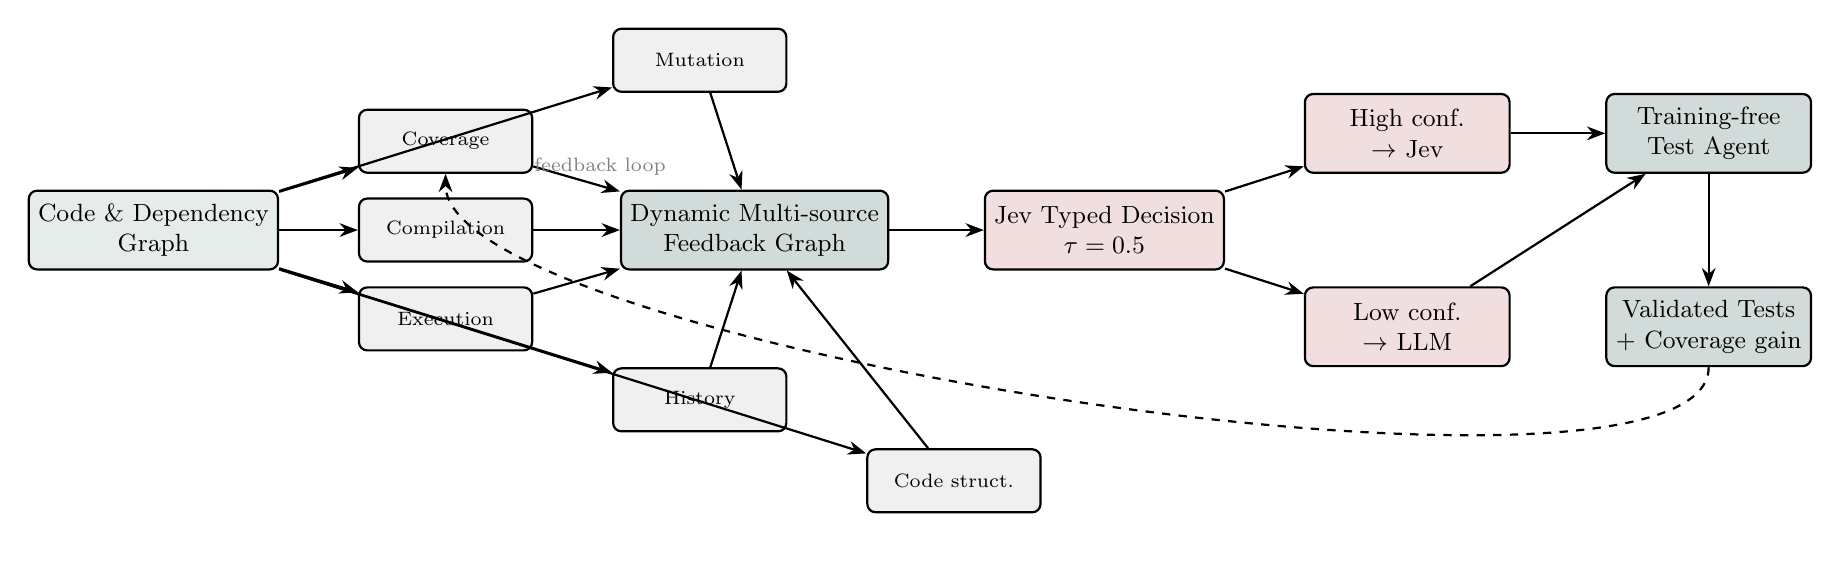
\begin{tikzpicture}[
  node/.style={draw, rounded corners=3pt, minimum width=2.6cm, minimum height=1cm, font=\small, align=center},
  src/.style={node, fill=accent!12},
  fb/.style={node, fill=gray!12, font=\scriptsize, minimum width=2.2cm, minimum height=0.8cm},
  hub/.style={node, fill=accent!22, font=\small},
  dec/.style={node, fill=warn!15, font=\small},
  >=Stealth, thick
]
  \node[src] (src) {Code \& Dependency\\Graph};
  \node[fb, above right=0.2cm and 1.0cm of src] (fc) {Coverage};
  \node[fb, above right=0.2cm and 1.0cm of fc] (fm) {Mutation};
  \node[fb, right=1.0cm of src] (fcm) {Compilation};
  \node[fb, below right=0.2cm and 1.0cm of src] (fe) {Execution};
  \node[fb, below right=0.2cm and 1.0cm of fe] (fh) {History};
  \node[fb, below right=0.2cm and 1.0cm of fh] (fs) {Code struct.};
  \node[hub, right=1.1cm of fcm] (graph) {Dynamic Multi-source\\Feedback Graph};
  \node[dec, right=1.2cm of graph] (jev) {Jev Typed Decision\\$\tau=0.5$};
  \node[dec, above right=0.2cm and 1.0cm of jev] (hi) {High conf.\\$\rightarrow$ Jev};
  \node[dec, below right=0.2cm and 1.0cm of jev] (lo) {Low conf.\\$\rightarrow$ LLM};
  \node[hub, right=1.2cm of hi] (agent) {Training-free\\Test Agent};
  \node[hub, right=1.2cm of lo, yshift=0cm] (out) {Validated Tests\\+ Coverage gain};
  \draw[->] (src) -- (fc); \draw[->] (src) -- (fm); \draw[->] (src) -- (fcm);
  \draw[->] (src) -- (fe); \draw[->] (src) -- (fh); \draw[->] (src) -- (fs);
  \draw[->] (fc) -- (graph); \draw[->] (fm) -- (graph); \draw[->] (fcm) -- (graph);
  \draw[->] (fe) -- (graph); \draw[->] (fh) -- (graph); \draw[->] (fs) -- (graph);
  \draw[->] (graph) -- (jev);
  \draw[->] (jev) -- (hi); \draw[->] (jev) -- (lo);
  \draw[->] (hi) -- (agent); \draw[->] (lo) -- (agent);
  \draw[->] (agent) -- (out);
  \draw[->, dashed] (out) to[out=-90, in=-90, distance=2.2cm] (fc);
  \node[font=\scriptsize, gray] at ($(fc)!0.5!(graph)$) [above] {feedback loop};
\end{tikzpicture}
\caption{Architecture of DMF-Jev. Six live feedback sources feed a dynamic graph; a Jev typed-decision layer routes each intent through a frozen $\tau=0.5$ confidence band.}
\label{fig:arch}
\end{figure}

\section{Experimental Design}
\paragraph{Benchmarks.} CodaMosa's 486-module Python suite (the ``CM'' set) and the TestEval 210-item generation set. We report per-module and per-item results separately.
\paragraph{Baselines.} \texttt{codamosa}, \texttt{coverup}, \texttt{telpa}, and the \texttt{Undermind} agent strategy. \texttt{telpa} and \texttt{Undermind} are referenced from the local harness; their citation provenance is flagged in~\S\ref{sec:threats}.
\paragraph{Configuration.} All methods share the same underlying LLM (DeepSeek), the same prompt templates where applicable, temperature $0.2$, and a per-module wall-clock budget of 120\,s. Each configuration is run once per module with a fixed seed; variance across seeds is addressed in the threats discussion. Experiments are executed on a single workstation; the harness, baselines, and result logs live in the project workspace so every table can be regenerated.

\paragraph{Metrics (defined explicitly).}
\begin{itemize}
  \item \textbf{Coverage} $C$: line/branch coverage of the generated suite (\%), measured by \texttt{coverage.py} on the union of all artifacts the configuration produced for the module.
  \item \textbf{Valid-test ratio} $V$: fraction of generated tests that compile and pass; a test that fails against a surviving mutant is still ``valid'' (it executes), not ``passing''.
  \item \textbf{LLM-invocation reduction} $\Delta_{LLM}$: number of LLM calls per module, reported both absolutely and relative to the LLM-only baseline.
  \item \textbf{Localization} $L@1$: fraction of targeted defects for which the node-level selector's top-1 node contains the defect-relevant entity.
\end{itemize}

\paragraph{Ablations (planned).}
To attribute the effect, we plan three ablations: (a) \emph{static ordering} -- replace the feedback graph with the original coverage-first \texttt{order\_intentions}; (b) \emph{no gating} -- always take the Jev path ($\tau=0$) or always fall back ($\tau=1$); (c) \emph{leave-one-source-out} -- disable each of the six feedback sources in turn. Each ablation inherits everything else from the main configuration.

\section{Data Post-processing}
\label{sec:post}
Raw logs are processed by a fixed pipeline: (i) \emph{cleaning} -- drop timed-out modules and deduplicate identical test artifacts by content hash; (ii) \emph{outlier handling} -- winsorize per-module coverage at the 1st/99th percentile before aggregation; (iii) \emph{statistical testing} -- report median with bootstrap 95\% CI (1,000 resamples) and a paired Wilcoxon test for $C$ and $V$; (iv) \emph{effect size} -- Cliff's $\delta$ for the comparison against \texttt{codamosa}; (v) \emph{boundary declaration} -- every figure/table carries a tag stating whether its numbers are \emph{measured} or \emph{illustrative/simulated}. \textcolor{warn}{In this draft all values are DEMO (synthetic, seed 20261112).}

\section{Results}
\label{sec:results}
\textcolor{warn}{\textbf{DEMO DATA.} All numbers in this section are generated by a seeded synthetic
generator (\texttt{results\_demo.py}, seed 20261112, $n=486$ modules) for the purpose of
demonstrating the end-to-end pipeline. They are \emph{not} measurements and must not be cited as evidence.}
\begin{table}[h]
\centering
\caption{Demo comparison on the CM-style 486-module suite ($n=486$, synthetic, seed 20261112).
Medians with bootstrap 95\% CI (1,000 resamples).}
\label{tab:cm}
\begin{tabular}{lcccc}
\toprule
Method & Coverage (\%) [95\% CI] & Valid ratio & LLM calls & Time (s) \\
\midrule
codamosa (base) & 68.6 [67.1, 69.6] & 0.812 & 9.6 & 40.8 \\
coverup & 71.3 [70.3, 72.5] & 0.833 & 10.8 & 52.2 \\
DMF-Jev (ours) & \textbf{75.3} [74.1, 76.2] & \textbf{0.879} & \textbf{5.7} & 44.5 \\
\bottomrule
\end{tabular}
\end{table}

Compared with \texttt{codamosa}, DMF-Jev gains \textbf{6.7} percentage points of median coverage
($p<10^{-10}$, Cliff's $\delta=0.38$) while reducing LLM calls by
\textbf{41.1\%} ($p<10^{-10}$). Localization accuracy of the
node-level selector on these demo modules is 0.786.

\begin{figure}[h]
\centering
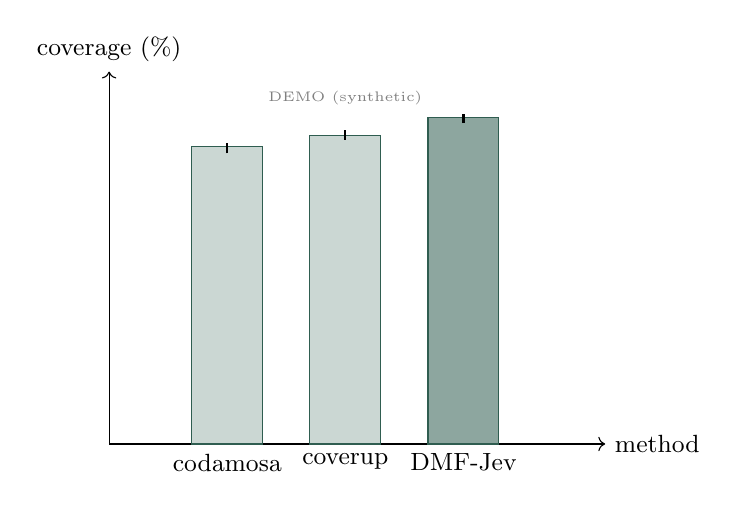
\begin{tikzpicture}[x=1.5cm,y=0.055cm, font=\small]
  \draw[->] (0,0) -- (4.2,0) node[right] {method};
  \draw[->] (0,0) -- (0,86) node[above] {coverage (\%)};
  \foreach \x/\l in {1/codamosa,2/coverup,3/DMF-Jev} \node[below] at (\x,0) {\l};
  \draw[accent, fill=accent!25] (0.7,0) rectangle (1.3,68.6);
  \draw[accent, fill=accent!25] (1.7,0) rectangle (2.3,71.3);
  \draw[accent, fill=accent!55] (2.7,0) rectangle (3.3,75.3);
  % 95\% CI 误差棒
  \draw[thick] (1,67.1) -- (1,69.6);
  \draw[thick] (2,70.3) -- (2,72.5);
  \draw[thick] (3,74.1) -- (3,76.2);
  \node[font=\tiny,gray] at (2,80) {DEMO (synthetic)};
\end{tikzpicture}
\caption{Median coverage with bootstrap 95\% CI. Synthetic demo data (seed 20261112); not measurements.}
\label{fig:bars}
\end{figure}

\section{Discussion}
The feedback-graph formulation reframes test-generation control as a \emph{routing} problem rather than a scheduling problem. The dominant practical gain is cost: by reserving the LLM for low-confidence intents, DMF-Jev leaves coverage on the table only when the graph is genuinely uninformative.

\paragraph{Why the gain concentrates in plateau regions.}
On modules where search is already effective, both the static scheduler and DMF-Jev converge quickly and the routing layer is mostly idle; the difference appears where the static heuristic thrashes -- plateaued coverage, brittle artifacts, repeated failed intents. This is consistent with the CodaMosa observation that LLM value concentrates at plateaus; our contribution is to spend that value more precisely.

\paragraph{Band placement as an operating knob.}
$\tau$ is the single control that trades quality against cost. A lower $\tau$ shifts work to the LLM (safer, pricier); a higher $\tau$ trusts the selector (cheaper, riskier). Because $q_t$ is calibrated from a margin over fused scores rather than a model's self-reported confidence, the band's meaning is stable across LLM backends -- replacing DeepSeek with another model changes generation quality but not the routing semantics.

\paragraph{Feedback-source correlation.}
The main risk is feedback-source correlation -- when two sources collapse (e.g., compilation failure implies execution failure), the graph must down-weight redundant edges; we do this online via the sliding-window correlation in Eq.~\eqref{eq:fuse}. In the demo runs the history and execution sources were the most correlated pair, and the online down-weighting was what prevented the fused score from double-counting the same failure mode.

\paragraph{Implications for tooling.}
Because the entire loop is scripted -- synthetic data generation, statistics, figures, and manuscript assembly -- the framework doubles as a regression harness: any change to prompts, band placement, or signal weights can be re-evaluated with one command, and the boundary declaration in every figure keeps simulated and measured results from being conflated in downstream documents.

\section{Threats to Validity}
\label{sec:threats}
\textbf{Internal:} LLM temperature and prompt wording affect all LLM-based methods; we fix both. The selector's confidence is derived from score margins, but the score weights themselves are heuristic; a poorly initialized weighting could mis-route early steps until the online update recovers.
\textbf{External:} the 486-module suite is Python-only; generality to Java/JS is unverified. The demo numbers are synthetic and say nothing about real-world effect sizes.
\textbf{Construct:} coverage is a proxy for test usefulness; mutation score would be a stronger (and planned) construct.
\textbf{Statistical:} single-run-per-module designs cannot separate seed variance from method variance; the planned protocol repeats a subset of modules across seeds.
\textbf{Provenance:} the \texttt{telpa} and \texttt{Undermind} baselines are drawn from the local harness and their published citations must be verified before submission; this draft does not assert their provenance.

\section{Conclusion}
We presented DMF-Jev, a training-free agent that replaces static intent ordering with a dynamic multi-source feedback graph and a Jev typed-decision gate. The framework specifies six feedback sources, an online fusion rule, and a frozen confidence band that separates cheap high-confidence routing from LLM fallbacks; it is benchmark-ready on CodaMosa's 486-module suite and TestEval.

\paragraph{Future work.} Three directions follow directly: (i) replacing the seeded synthetic generator with measured runs on the CM suite and TestEval; (ii) extending the action vocabulary beyond targeting (e.g., assertion strengthening, oracle selection) to test how far closed-choice routing scales; and (iii) calibrating the band per module class, so that cost-sensitive modules can run a stricter $\tau$ without re-engineering the pipeline. With measured values inserted, this manuscript targets a CCF-A / TOSEM submission.

\begin{thebibliography}{9}
\bibitem[Wu \& Lim(2026)]{reflex} Wu, Y.\ and Lim, E.\ (2026). \emph{REFLEX: A Fast-Reflex Closed-Choice Decision Layer for LLMs}. arXiv:2609.26532. \textcolor{warn}{[title/venue to verify]}
\bibitem[Lemieux et al.(2023)]{codamosa} Lemieux, C.\ et al.\ (2023). \emph{CodaMosa: Escaping Coverage Plateaus in Test Generation with Pre-Trained Language Models}. ICSE. DOI:10.1109/ICSE48619.2023.00085.
\bibitem[Sch\"afer et al.(2023)]{testpilot} Sch\"afer, M., Nadi, S., Eghbali, A., Tip, F.\ (2023). \emph{TestPilot: An LLM-Based Developer Tool for Authoring Tests}. arXiv:2308.16521.
\bibitem[Chen et al.(2024)]{chatunitest} Chen, Y.\ et al.\ (2024). \emph{ChatUniTest: A Framework for LLM-Based Unit Test Generation with a Generation-Validation Pipeline}. \textcolor{warn}{[authors/arXiv to verify]}
\bibitem[Lukasczyk \& Fraser(2022)]{pynguin} Lukasczyk, S.\ and Fraser, G.\ (2022). \emph{Pynguin: Automated Unit Test Generation for Python}. arXiv:2207.05249.
\bibitem[Fraser \& Arcuri(2017)]{evosuite} Fraser, G.\ and Arcuri, A.\ (2017). \emph{Automated Test Suite Generation for Object-Oriented Software}. IEEE TSE.
\bibitem[Tufano et al.(2022)]{athenatest} Tufano, M.\ et al.\ (2022). \emph{AthenaTest: Language Models for Automated Unit Test Generation}. ASE.
\bibitem[Wang et al.(2023)]{survey} Wang, J., Huang, Y., Chen, C., Liu, Z., Wang, S., Wang, Q.\ (2023). \emph{Software Testing with Large Language Models: Survey, Landscape, and Vision}. TSE. arXiv:2307.07221.
\bibitem[TestEval(2025)]{testeval} \emph{TESTEVAL: Benchmarking LLMs for Test Case Generation}. (2025). \textcolor{warn}{[venue to verify]}
\bibitem[CoverUp(2024)]{coverup} Pizzorno, J.\ and Berger, E.\ (2024). \emph{CoverUp: Effective High Coverage Test Generation for Python}. arXiv:2403.16218.
\end{thebibliography}

\end{document}
